\chapter{Noten}
\label{noten}
\begin{figure}
	\centering
	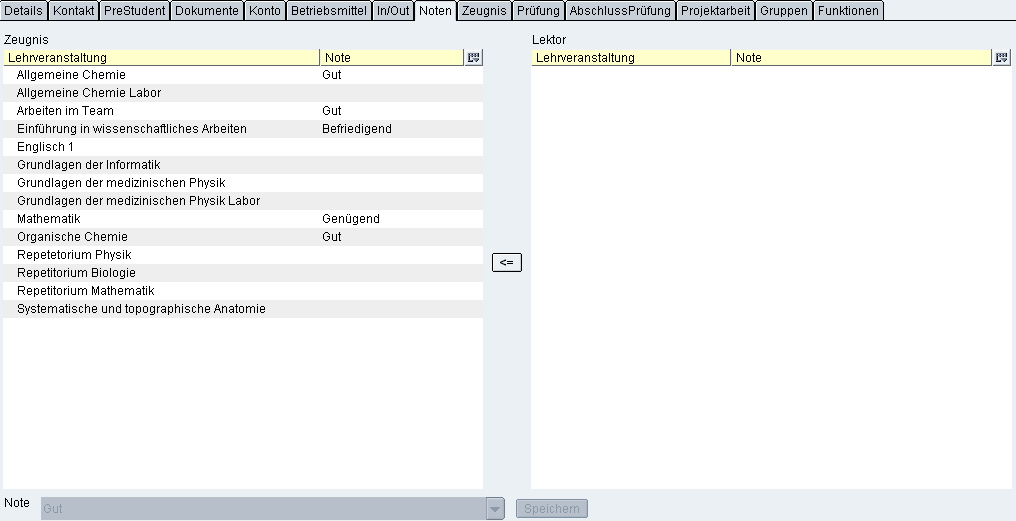
\includegraphics[width=0.75\textwidth]{FAS_Noten1.png}
	\caption{Die Karteikarte Noten}
	\label{noten1}
\end{figure}
\section{Aufbau der Karteikarte}
\begin{itemize}
	\item Listenfeld links: In diesem Fenster befinden sich alle Lehrveranstaltungen, denen der Student indirekt �ber Gruppen zugeordnet ist. Die hier eingetragenen Noten scheinen auf dem Semesterzeugnis auf sofern das die Lehrveranstaltungseinstellugen zulassen.
	\item Listenfeld rechts: Hier werden die aktuellen Noten, die die Lektoren eingegeben haben, angezeigt. Unterscheiden sich Noten von denen der gleichen Lehrveranstaltung im linken Listenfeld, wird die betreffende Zeile vorselektiert.
	\item Button <=: �bertragen von Noten vom Lektoreneintrag in die Liste der Zeugnisnoten.
\end{itemize}
\section{Noteneingabe und -�bergabe}
Einzelne Noten k�nnen in der Karteikarte \textit{Noten} eingetragen werden. Dazu befindet sich am unteren Rand der Karteikarte ein Auswahlfeld in dem die Note der im linken Listenfeld ausgew�hlten Lehrveranstaltung bestimmt werden kann. \\
Noten k�nnen aber auch vom Lektor auf der CIS-Seite eingegeben werden. Die aktuellste Eintragungen scheinen dann in der rechten Liste auf. Unterscheiden sich Noten von bereits �bernommenen, werden sie vorselektiert angezeigt und k�nnen direkt durch Klicken der \textit{<=}-Taste �bernommen werden. Wurde eine Lehrveranstaltung dem Studenten angerechnet, kann diese Eintragung nur manuell ge�ndert werden.\\
Es besteht auch eine M�glichkeit, die Noten einer Lehrveranstaltung zu �bernehmen, ohne jeden Studenten einzeln aufrufen zu m�ssen. Dazu �ffnet man im Listenfeld 2 die entsprechende Lehrveranstaltung und wechselt im Datenfeld dann in die Karteikarte \textit{Noten}. Hier werden in der linken Liste die an der Lehrveranstaltung teilnehmenden Studenten und im rechten Listenfeld die Studenten mit der vom Lektor zuletzt eingetragenen Note aufgelistet. Um die Noten zu �bernehmen, werden die entsprechenden Zeilen in der rechten Liste markiert und mit der \textit{<=}-Taste in die linke Liste kopiert.\\

\info{Wenn die Assistenz eine Note ver�ndert (bspw die Note einer Nachpr�fung eintr�gt) dann wird die Note des Lektors nicht mehr zur �bernahme markiert auch wenn diese dann unterschiedlich zur Zeugnisnote ist. (d.h. wenn das Benotungsdatum der Zeugnisnote j�nger ist als das Benotungsdatum des Lektors)}\\
